\begin{figure*}[t]
\centering
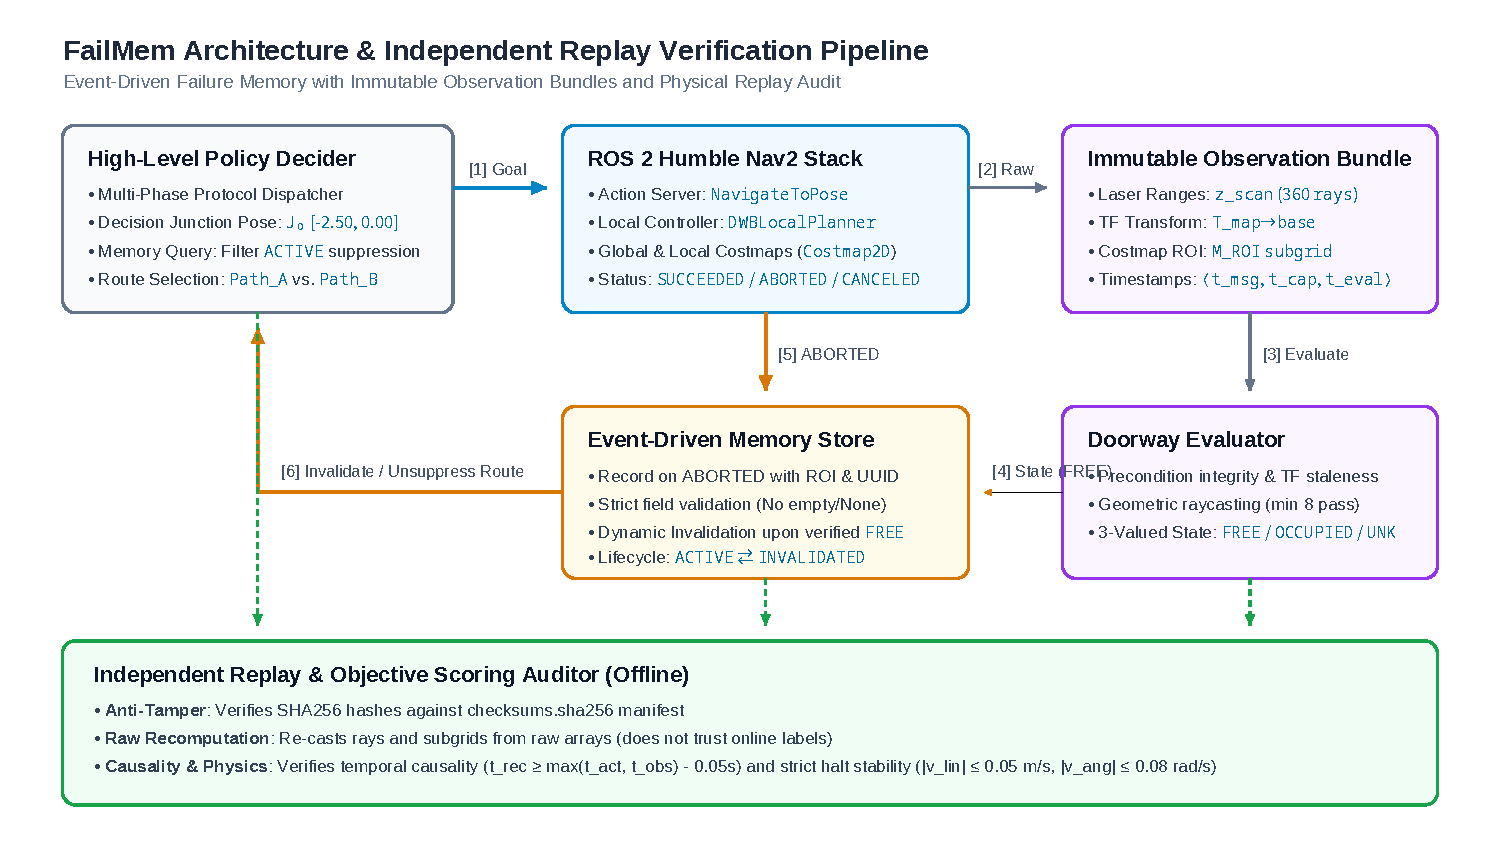
\includegraphics[width=0.85\textwidth]{figures/architecture.pdf}
\caption{FailMem system architecture and verification pipeline, encompassing execution runtime, immutable observation bundles, and memory lifecycle.}
\label{fig:architecture}
\end{figure*}

Figure~\ref{fig:architecture} illustrates the overall system architecture, encompassing the execution runtime, immutable observation bundles, and memory lifecycle.

\subsection{Immutable Observation Bundles}
Prior to evaluating passage clearance, FailMem constructs an immutable observation bundle $B$:
\begin{equation}
B = \langle \text{obs\_id}, \mathbf{z}_{\text{scan}}, \mathbf{T}_{\text{map}\to\text{base}}, \mathbf{M}_{\text{costmap\_ROI}}, t_{\text{msg}}, t_{\text{capture}}, t_{\text{eval}} \rangle
\end{equation}
where $\mathbf{z}_{\text{scan}}$ is the raw range array, $\mathbf{T}_{\text{map}\to\text{base}}$ is the TF transformation, and $\mathbf{M}_{\text{costmap\_ROI}}$ is the extracted 2D subgrid matrix.

\subsection{Clearance Classification Rules}
The passage state is evaluated according to strict geometric criteria implemented in \texttt{src/doorway\_evaluator.py}:
\begin{equation}
\text{State}(B) = \begin{cases} 
\text{OCCUPIED}, & \text{if } N_{\text{hits\_inside}} \ge 5 \text{ or } N_{\text{costmap\_occupied\_cells}} > 0 \\ 
\text{FREE}, & \text{if } N_{\text{hits\_inside}} = 0 \text{ and } N_{\text{pass\_through}} \ge 8 \\
             & \quad \text{and } \text{CostmapCleared}(B) \\ 
\text{UNKNOWN}, & \text{otherwise} 
\end{cases}
\end{equation}
where $\text{CostmapCleared}(B) \iff (N_{\text{unknown\_cells}} = 0 \land N_{\text{occupied\_cells}} = 0)$ within the doorway ROI $[-0.15, 0.15, 0.95, 1.45]$. (See Supplementary Material S1 for detailed transform alignment and ray projection preconditions).

\subsection{Memory Lifecycle \& Invalidation Mechanics}
\begin{itemize}
    \item \textbf{Failure Registration}: When navigation fails within an occupied passage, an active failure record is created:
    \begin{equation}
    M = \langle \text{mem\_id}, t_{\text{fail}}, \text{goal\_uuid}, \text{action\_id}, \text{region\_id}, \mathbf{M}_{\text{costmap\_ROI}} \rangle
    \end{equation}
    Active failure records suppress the associated route at Decision Junction $J_0$.
    \item \textbf{Dynamic Invalidation}: When subsequent sensor perception yields $\text{State}(B) = \text{FREE}$ with evidence timestamp $t_{\text{free}} > t_{\text{fail}}$, the memory entry is marked $\text{INVALIDATED}$, unsuppressing the route.
    \item \textbf{Cross-Phase Scope Clarification}: In the current experimental implementation, history collection, memory creation, decision dispatch, and memory reset occur within a single continuous runner session across sequential phases. This evaluates phase-to-phase memory transfer within an experimental run, and has not yet been benchmarked as a persistent multi-task database across separate OS daemon lifetimes.
    \item \textbf{Evaluation Pipeline}: An independent replay auditor verifies all serialized logs against SHA256 checksum manifests (detecting file changes relative to the manifest) and physical halt stability criteria ($|v_{\text{lin}}| \le 0.05\,\text{m/s}, |v_{\text{ang}}| \le 0.08\,\text{rad/s}$) without reliance on self-reported runtime assertions (detailed in Supplementary Material Section S2).
\end{itemize}
